\documentclass[12pt,a4paper]{article}

% ============================================================
% PACKAGES
% ============================================================
\usepackage[utf8]{inputenc}
\usepackage[T1]{fontenc}
\usepackage{mathpazo}                   % Palatino font (journal standard)
\usepackage[margin=1in]{geometry}
\usepackage{setspace}\onehalfspacing
\usepackage{amsmath,amssymb}
\usepackage{booktabs}                   % Professional tables
\usepackage{tabularx}
\usepackage{multirow}
\usepackage{threeparttable}             % Table notes
\usepackage{graphicx}
\usepackage{float}
\usepackage[labelfont=bf,font=small]{caption}
\usepackage{natbib}                     % Bibliography
\usepackage[hidelinks]{hyperref}
\usepackage{xcolor}
\usepackage{enumitem}
\usepackage{pdflscape}                  % Landscape pages

% ============================================================
% TITLE
% ============================================================
\title{\textbf{Revolution and Reproduction: \\[6pt] How the Arab Spring Reshaped Marriage and Fertility in Egypt} \\[12pt]
\large Summary of Empirical Results}

\author{Yeganeh Karbalaei\thanks{Department of Economics, University of Oklahoma.} \and Firat Demir\thanks{Department of Economics, University of Oklahoma.} \and Pallab Ghosh\thanks{Department of Economics, University of Oklahoma. Email: pghosh@ou.edu}}

\date{February 2026 \\ \small Draft 1 --- Results Summary}

\begin{document}

\maketitle

\begin{abstract}
\noindent We examine the consequences of the Arab Spring on women's reproductive and labor market outcomes in Egypt. We draw on three rounds of the Egypt Demographic and Health Survey (DHS 2005, 2008, 2014) and employ a difference in differences strategy that exploits geographic variation in exposure to the 2011 uprising. We find that Arab Spring exposure significantly reduced teen pregnancy rates, raised the age at first birth and first marriage, and shifted occupational composition away from unskilled manual labor. We trace these effects to two primary mechanisms---delayed marriage and a narrowing of the spousal age gap---while ruling out changes in education, partner selection, and labor force participation as operative channels. We subject our estimates to a battery of robustness checks, including a miscarriage placebo test and logit specifications. \\[6pt]
\noindent \textit{JEL Classification}: J13, J16, O15, I15 \\
\noindent \textit{Keywords}: Arab Spring, teen pregnancy, women's outcomes, difference in differences, Egypt
\end{abstract}

\newpage
\tableofcontents
\newpage

% ============================================================
% SECTION 1: INTRODUCTION
% ============================================================
\section{Introduction and Empirical Strategy}

\subsection{Trends in Teen Pregnancy}

We begin by documenting the trends in teen pregnancy rates for the treatment and control groups over the study period. Figure~\ref{fig:trends} plots these trends, with the dashed vertical line marking the onset of the Arab Spring in 2011.
\vspace{0.25cm}

\begin{figure}[H]
\centering
\begin{minipage}{0.48\textwidth}
    \centering
    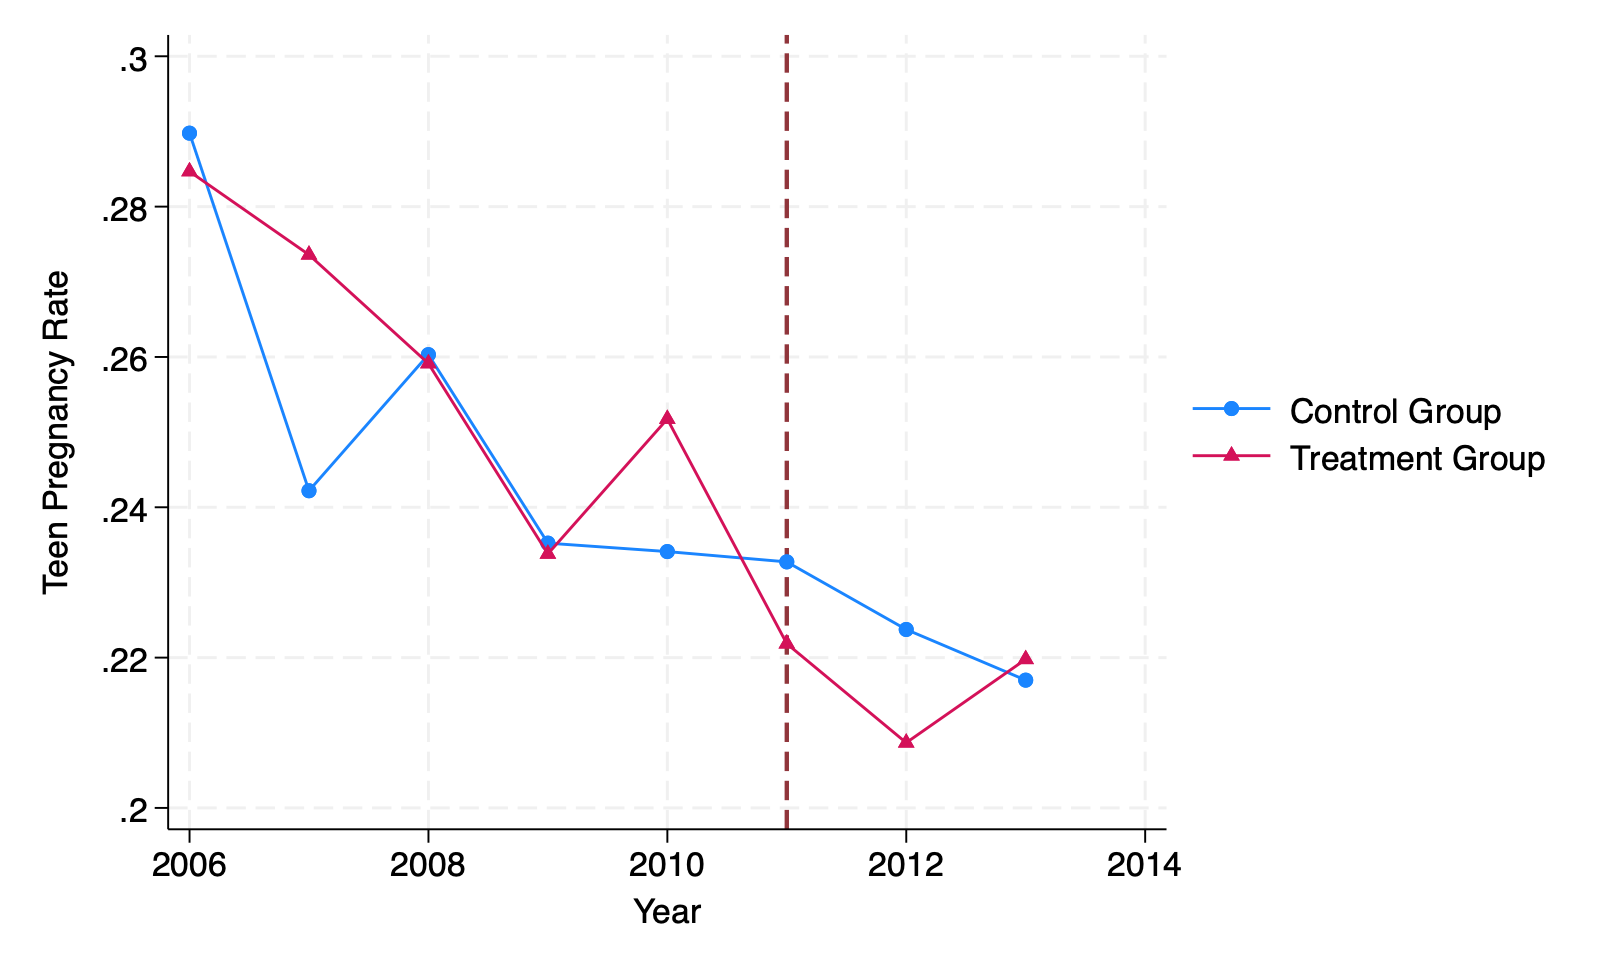
\includegraphics[width=\textwidth]{teen_preg_trends.png}
    \caption*{(a) Raw trends}
\end{minipage}
\hfill
\begin{minipage}{0.48\textwidth}
    \centering
    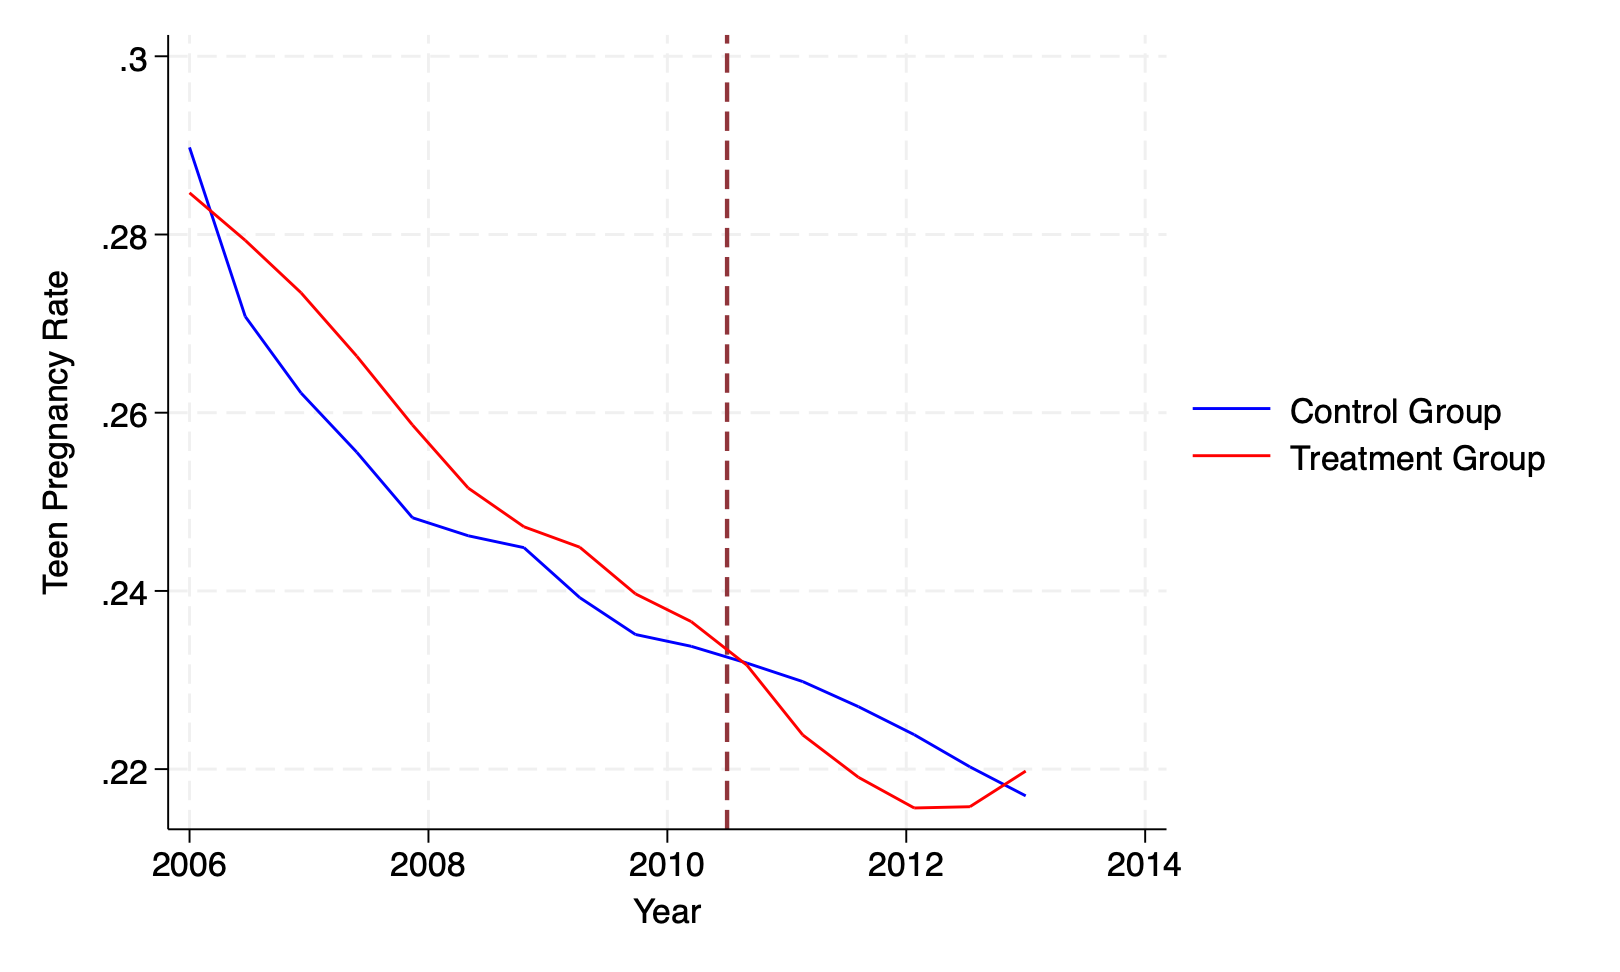
\includegraphics[width=\textwidth]{teen_preg_trends_smooth.png}
    \caption*{(b) Smoothed trends}
\end{minipage}
\caption{Teen Pregnancy Rates by Treatment and Control Groups, 2006--2014}
\label{fig:trends}
\end{figure}

\noindent Several features of Figure~\ref{fig:trends} are worth noting. First, the pre 2011 trends in teen pregnancy move broadly in parallel across treatment and control groups, lending support to our key identifying assumption. Second, after 2011, the treatment group experiences a noticeably steeper decline in teen pregnancy relative to the control group, consistent with a causal effect of the uprising. The smoothed trends in panel (b) make this post 2011 divergence especially visible.
\vspace{0.25cm}

\subsection{Summary Statistics}

Table~\ref{tab:sumstats} presents the summary statistics for the key variables used in our analysis. Panel~A reports the full sample, Panel~B compares treatment and control groups, and Panel~C shows means by survey year.
\vspace{0.25cm}

\begin{table}[H]
\centering
\begin{threeparttable}
\caption{Summary Statistics}
\label{tab:sumstats}
\small
\begin{tabular}{@{}lccccc@{}}
\toprule
\multicolumn{6}{@{}l}{\textit{Panel A: Full Sample}} \\[2pt]
Variable & $N$ & Mean & Std.\ Dev. & Min & Max \\
\midrule
Teen pregnancy           & 40,571 & 0.343 & 0.475 & 0 & 1 \\
Age at first birth       & 40,571 & 21.406 & 3.896 & 8 & 45 \\
Age at first marriage    & 40,571 & 19.816 & 3.872 & 8 & 44 \\
No education             & 40,571 & 0.256 & 0.436 & 0 & 1 \\
Primary education        & 40,571 & 0.104 & 0.305 & 0 & 1 \\
Secondary education      & 40,571 & 0.513 & 0.500 & 0 & 1 \\
Respondent age           & 40,571 & 28.524 & 5.834 & 15 & 49 \\
Respondent works         & 40,524 & 0.142 & 0.367 & 0 & 9 \\
Husband age              & 40,571 & 35.174 & 7.656 & 14 & 95 \\
Husband works            & 40,226 & 0.982 & 0.131 & 0 & 1 \\
Husband no education     & 40,571 & 0.160 & 0.367 & 0 & 1 \\
Husband primary          & 40,571 & 0.155 & 0.362 & 0 & 1 \\
Husband secondary        & 40,571 & 0.533 & 0.499 & 0 & 1 \\
Poorest                  & 40,571 & 0.219 & 0.414 & 0 & 1 \\
Poorer                   & 40,571 & 0.202 & 0.401 & 0 & 1 \\
Middle                   & 40,571 & 0.204 & 0.403 & 0 & 1 \\
Richer                   & 40,571 & 0.193 & 0.395 & 0 & 1 \\
Birth order              & 40,571 & 2.602 & 1.699 & 1 & 19 \\
Religion (Muslim)        & 40,539 & 0.960 & 0.196 & 0 & 1 \\
Terminated birth         & 38,574 & 0.166 & 0.372 & 0 & 1 \\
TC\_noborder             & 38,183 & 0.458 & 0.498 & 0 & 1 \\
Post 2011 (Time dummy)   & 40,571 & 0.277 & 0.447 & 0 & 1 \\
\bottomrule
\end{tabular}
\begin{tablenotes}[flushleft]
\footnotesize
\item \textit{Notes}: Data from Egypt DHS 2005, 2008, and 2014. Teen pregnancy is defined as first birth before age 20. Wealth quintile reference category is Richest. Education reference is postsecondary.
\end{tablenotes}
\end{threeparttable}
\end{table}

\begin{table}[H]
\centering
\begin{threeparttable}
\caption{Summary Statistics by Treatment/Control Group and Survey Year}
\label{tab:sumstats_groups}
\small
\begin{tabular}{@{}lcccccc@{}}
\toprule
\multicolumn{7}{@{}l}{\textit{Panel B: By Treatment and Control Group}} \\[2pt]
 & \multicolumn{3}{c}{Treatment ($N = 17{,}489$)} & \multicolumn{3}{c}{Control ($N = 20{,}694$)} \\
\cmidrule(lr){2-4} \cmidrule(lr){5-7}
Variable & Mean & SD & & Mean & SD & \\
\midrule
Teen pregnancy         & 0.358 & 0.479 & & 0.334 & 0.472 & \\
Age at first birth     & 21.383 & 4.016 & & 21.398 & 3.785 & \\
Age at first marriage  & 19.838 & 4.000 & & 19.775 & 3.753 & \\
No education           & 0.270 & 0.444 & & 0.238 & 0.426 & \\
Primary education      & 0.108 & 0.310 & & 0.098 & 0.298 & \\
Secondary education    & 0.484 & 0.500 & & 0.545 & 0.498 & \\
Respondent age         & 28.481 & 5.874 & & 28.497 & 5.789 & \\
Respondent works       & 0.156 & 0.363 & & 0.129 & 0.361 & \\
Birth order            & 2.573 & 1.687 & & 2.606 & 1.696 & \\
\midrule
\multicolumn{7}{@{}l}{\textit{Panel C: By Survey Year}} \\[2pt]
 & \multicolumn{2}{c}{2005 ($N = 13{,}851$)} & \multicolumn{2}{c}{2008 ($N = 10{,}872$)} & \multicolumn{2}{c}{2014 ($N = 15{,}848$)} \\
\cmidrule(lr){2-3} \cmidrule(lr){4-5} \cmidrule(lr){6-7}
Variable & \multicolumn{2}{c}{Mean} & \multicolumn{2}{c}{Mean} & \multicolumn{2}{c}{Mean} \\
\midrule
Teen pregnancy         & \multicolumn{2}{c}{0.388} & \multicolumn{2}{c}{0.355} & \multicolumn{2}{c}{0.296} \\
Age at first birth     & \multicolumn{2}{c}{20.996} & \multicolumn{2}{c}{21.345} & \multicolumn{2}{c}{21.806} \\
Age at first marriage  & \multicolumn{2}{c}{19.340} & \multicolumn{2}{c}{19.734} & \multicolumn{2}{c}{20.288} \\
No education           & \multicolumn{2}{c}{0.334} & \multicolumn{2}{c}{0.279} & \multicolumn{2}{c}{0.171} \\
Primary education      & \multicolumn{2}{c}{0.126} & \multicolumn{2}{c}{0.102} & \multicolumn{2}{c}{0.085} \\
Secondary education    & \multicolumn{2}{c}{0.448} & \multicolumn{2}{c}{0.499} & \multicolumn{2}{c}{0.580} \\
Respondent age         & \multicolumn{2}{c}{28.479} & \multicolumn{2}{c}{28.370} & \multicolumn{2}{c}{28.668} \\
\bottomrule
\end{tabular}
\begin{tablenotes}[flushleft]
\footnotesize
\item \textit{Notes}: Treatment group defined by TC\_noborder $= 1$. Panel C reports unconditional means by DHS survey wave.
\end{tablenotes}
\end{threeparttable}
\end{table}

\begin{table}[H]
\centering
\begin{threeparttable}
\caption{Difference in Differences Summary Statistics}
\label{tab:did_sumstats}
\footnotesize
\begin{tabular}{@{}l cc@{\hspace{1.2em}}cc@{\hspace{1.2em}}c@{}}
\toprule
 & \multicolumn{2}{c}{Pre Period} & \multicolumn{2}{c}{Post Period} & \\
\cmidrule(lr){2-3} \cmidrule(lr){4-5}
Variable & Control & Treatment & Control & Treatment & DiD Estimate \\
\midrule
\multicolumn{6}{@{}l}{\textit{Panel A: Outcome Variables}} \\[1pt]
Teen pregnancy         & 0.350 & 0.380 & 0.294 & 0.297 & $-$0.027$^{**}$ \\
                       &       &       &       &       & ($-$2.521) \\[2pt]
Age at first birth     & 21.260 & 21.168 & 21.744 & 21.993 & 0.341$^{***}$ \\
                       &       &       &       &       & (3.744) \\[2pt]
Age at first marriage  & 19.613 & 19.584 & 20.180 & 20.559 & 0.408$^{***}$ \\
                       &       &       &       &       & (4.544) \\[4pt]
\multicolumn{6}{@{}l}{\textit{Panel B: Education}} \\[1pt]
No education           & 0.269 & 0.312 & 0.160 & 0.152 & $-$0.050$^{***}$ \\
                       &       &       &       &       & ($-$5.601) \\[2pt]
Primary education      & 0.106 & 0.118 & 0.079 & 0.081 & $-$0.010 \\
                       &       &       &       &       & ($-$1.470) \\[2pt]
Secondary education    & 0.521 & 0.450 & 0.604 & 0.578 & 0.045$^{***}$ \\
                       &       &       &       &       & (3.956) \\[4pt]
\multicolumn{6}{@{}l}{\textit{Panel C: Respondent and Household Characteristics}} \\[1pt]
Respondent age         & 28.727 & 28.579 & 27.920 & 28.202 & 0.430$^{***}$ \\
                       &       &       &       &       & (3.286) \\[2pt]
Respondent works       & 0.135 & 0.166 & 0.114 & 0.127 & $-$0.018$^{**}$ \\
                       &       &       &       &       & ($-$2.289) \\[2pt]
Husband age            & 35.700 & 35.407 & 34.141 & 34.101 & 0.253 \\
                       &       &       &       &       & (1.495) \\[2pt]
Husband works          & 0.980 & 0.981 & 0.989 & 0.989 & $-$0.001 \\
                       &       &       &       &       & ($-$0.247) \\[2pt]
Husband no education   & 0.164 & 0.191 & 0.117 & 0.121 & $-$0.022$^{***}$ \\
                       &       &       &       &       & ($-$2.847) \\[2pt]
Birth order            & 2.655 & 2.625 & 2.481 & 2.426 & $-$0.025 \\
                       &       &       &       &       & ($-$0.712) \\[2pt]
Religion (Muslim)      & 0.959 & 0.955 & 0.964 & 0.968 & 0.008$^{*}$ \\
                       &       &       &       &       & (1.810) \\[4pt]
\multicolumn{6}{@{}l}{\textit{Panel D: Robustness Outcome}} \\[1pt]
Terminated birth       & 0.156 & 0.155 & 0.207 & 0.190 & $-$0.017$^{*}$ \\
                       &       &       &       &       & ($-$1.817) \\
\bottomrule
\end{tabular}
\begin{tablenotes}[flushleft]
\scriptsize
\item \textit{Notes}: Pre period includes DHS 2005 and 2008; post period is DHS 2014. Treatment/control defined by TC\_noborder. DiD estimate is the coefficient on Treatment $\times$ Post with robust standard errors. $t$ statistics in parentheses. $^{***}$~$p<0.01$, $^{**}$~$p<0.05$, $^{*}$~$p<0.10$.
\end{tablenotes}
\end{threeparttable}
\end{table}

\noindent Several patterns emerge from the descriptive statistics. About 34.3\% of women in our sample experienced teen pregnancy, with an average age at first birth of 21.4 years and first marriage of 19.8 years (Table~\ref{tab:sumstats}). The treatment and control groups are broadly balanced on observables---ages, birth orders, and marriage ages are similar---supporting the validity of the DiD design. Furthermore, teen pregnancy rates decline monotonically across survey waves, from 38.8\% in 2005 to 29.6\% in 2014, while the age at first marriage rises from 19.3 to 20.3 years. Educational composition also improves steadily: the share with no education falls from 33.4\% to 17.1\%, while secondary education rises from 44.8\% to 58.0\%. The sample is 96\% Muslim, with 27.7\% observed in the post 2011 period and 45.8\% in the treatment group.
\vspace{0.25cm}

Table~\ref{tab:did_sumstats} presents the unconditional difference in differences for each variable. Even without controlling for covariates, the raw DiD estimates show statistically significant effects on key outcomes: teen pregnancy declines by 2.7 percentage points ($t = -2.52$), age at first birth increases by 0.34 years ($t = 3.74$), and age at first marriage increases by 0.41 years ($t = 4.54$). Importantly, several control variables---husband's age, husband's work status, and birth order---show insignificant DiD estimates, suggesting that these characteristics did not differentially change between treatment and control groups around the Arab Spring. The terminated birth outcome also shows only marginal significance ($t = -1.82$), foreshadowing the robustness results in Section~5.
\vspace{0.25cm}

\subsection{Empirical Framework}

In this paper we use three rounds of the Egypt Demographic and Health Survey (DHS)---2005, 2008, and 2014---providing a combined sample of approximately 40,500 women (see Table~\ref{tab:sumstats}). Our identification strategy relies on a difference in differences framework that exploits variation in the intensity of Arab Spring exposure across Egyptian governorates. As shown in Figure~\ref{fig:trends}, the pretreatment trends in teen pregnancy are broadly parallel, supporting our identifying assumption. The key treatment variables are:

\begin{itemize}[nosep]
    \item \textbf{past\_group}: A measure of exposure to the Arab Spring, capturing whether women in a given governorate experienced the uprising during a critical period.
    \item \textbf{TC\_noborder}: The DiD estimator, interacting treatment status with the post period and excluding border governorates to ensure cleaner identification.
\end{itemize}

\noindent We estimate progressively controlled specifications to assess the sensitivity of our treatment effects:
\begin{enumerate}[nosep]
    \item \textbf{Specification (1)}: Baseline with wealth controls only
    \item \textbf{Specification (2)}: Adding respondent's education and age
    \item \textbf{Specification (3)}: Adding husband's characteristics
    \item \textbf{Specification (4)}: Adding birth order and religion
    \item \textbf{Specification (5)}: Full model with all controls
\end{enumerate}
\vspace{0.25cm}

% ============================================================
% SECTION 2: MAIN ESTIMATION
% ============================================================
\section{Main Estimation Results}

\subsection{Teen Pregnancy: All Specifications}

Table~\ref{tab:teen_preg} reports the full specification results for teen pregnancy, our primary outcome variable. The coefficient on \texttt{past\_group} is robustly negative across all five specifications, declining from $-$0.203 in the baseline to $-$0.095 in the full model as controls are progressively added. This attenuation is expected: controlling for education, age, and birth order absorbs some of the treatment effect that operates through these channels.
\vspace{0.25cm}

\begin{table}[H]
\centering
\begin{threeparttable}
\caption{Teen Pregnancy: Progressive Specifications}
\label{tab:teen_preg}
\footnotesize
\begin{tabular}{@{}lccccc@{}}
\toprule
 & (1) & (2) & (3) & (4) & (5) \\
 & Baseline & + Respondent & + Husband & + Birth Order & Full Model \\
\midrule
\multicolumn{6}{@{}l}{\textit{Treatment Variables}} \\[1pt]
past\_group  & $-$0.203$^{***}$ & $-$0.048$^{***}$ & $-$0.226$^{***}$ & $-$0.099$^{***}$ & $-$0.095$^{***}$ \\
             & (0.013) & (0.012) & (0.013) & (0.011) & (0.011) \\[2pt]
TC\_noborder & 0.133$^{***}$ & 0.061$^{***}$ & 0.133$^{***}$ & 0.068$^{***}$ & 0.067$^{***}$ \\
             & (0.013) & (0.010) & (0.013) & (0.008) & (0.008) \\[4pt]
\multicolumn{6}{@{}l}{\textit{Wealth Controls (ref: Richest)}} \\[1pt]
Poorest      & 0.335$^{***}$ & 0.143$^{***}$ & 0.258$^{***}$ & 0.032$^{***}$ & 0.033$^{***}$ \\
             & (0.013) & (0.013) & (0.014) & (0.012) & (0.012) \\[2pt]
Poorer       & 0.266$^{***}$ & 0.099$^{***}$ & 0.201$^{***}$ & 0.027$^{**}$ & 0.026$^{**}$ \\
             & (0.013) & (0.013) & (0.014) & (0.011) & (0.011) \\[2pt]
Middle       & 0.192$^{***}$ & 0.072$^{***}$ & 0.141$^{***}$ & 0.016 & 0.014 \\
             & (0.012) & (0.012) & (0.012) & (0.010) & (0.010) \\[2pt]
Richer       & 0.098$^{***}$ & 0.027$^{***}$ & 0.063$^{***}$ & $-$0.004 & $-$0.005 \\
             & (0.010) & (0.010) & (0.011) & (0.009) & (0.009) \\[4pt]
\multicolumn{6}{@{}l}{\textit{Respondent Characteristics}} \\[1pt]
Resp.\ work      &  $-$0.050$^{***}$ & 0.005 & $-$0.029$^{***}$ & 0.017$^{**}$ & 0.020$^{***}$ \\
                  & (0.008) & (0.008) & (0.008) & (0.007) & (0.007) \\[2pt]
No education     & & 0.336$^{***}$ & & 0.209$^{***}$ & 0.186$^{***}$ \\
                  & & (0.011) & & (0.010) & (0.012) \\[2pt]
Primary edu.     & & 0.340$^{***}$ & & 0.226$^{***}$ & 0.203$^{***}$ \\
                  & & (0.013) & & (0.012) & (0.013) \\[2pt]
Secondary edu.   & & 0.186$^{***}$ & & 0.121$^{***}$ & 0.105$^{***}$ \\
                  & & (0.007) & & (0.007) & (0.008) \\[2pt]
Resp.\ age       & & $-$0.027$^{***}$ & & $-$0.049$^{***}$ & $-$0.054$^{***}$ \\
                  & & (0.001) & & (0.001) & (0.001) \\[4pt]
\multicolumn{6}{@{}l}{\textit{Husband Characteristics}} \\[1pt]
Husband work     & & & 0.037 & & 0.014 \\
                  & & & (0.027) & & (0.023) \\[2pt]
Husb.\ no edu.   & & & 0.182$^{***}$ & & 0.029$^{**}$ \\
                  & & & (0.014) & & (0.013) \\[2pt]
Husb.\ primary   & & & 0.172$^{***}$ & & 0.035$^{***}$ \\
                  & & & (0.011) & & (0.012) \\[2pt]
Husb.\ secondary & & & 0.106$^{***}$ & & 0.023$^{***}$ \\
                  & & & (0.009) & & (0.009) \\[2pt]
Husband age      & & & 0.006$^{***}$ & & 0.007$^{***}$ \\
                  & & & (0.001) & & (0.001) \\[4pt]
\multicolumn{6}{@{}l}{\textit{Other Controls}} \\[1pt]
Birth order      & & & & 0.158$^{***}$ & 0.153$^{***}$ \\
                  & & & & (0.002) & (0.002) \\[2pt]
Religion         & & & & 0.003 & 0.004 \\
                  & & & & (0.015) & (0.015) \\[2pt]
Constant         & 0.130$^{***}$ & 0.809$^{***}$ & $-$0.194$^{***}$ & 1.163$^{***}$ & 1.043$^{***}$ \\
                  & (0.010) & (0.037) & (0.037) & (0.035) & (0.042) \\[3pt]
\midrule
Observations     & 38,118 & 38,118 & 37,793 & 38,087 & 37,762 \\
Adj.\ $R^2$      & 0.195  & 0.253  & 0.212  & 0.395  & 0.401 \\
\bottomrule
\end{tabular}
\begin{tablenotes}[flushleft]
\scriptsize
\item \textit{Notes}: Dependent variable is an indicator for teen pregnancy. Standard errors in parentheses. Reference categories: Richest (wealth), Postsecondary education (respondent and husband). $^{***}$~$p<0.01$, $^{**}$~$p<0.05$, $^{*}$~$p<0.10$.
\end{tablenotes}
\end{threeparttable}
\end{table}

\noindent The progressive inclusion of controls reveals several important patterns. Moving from Specification~(1) to~(2), the addition of respondent's education and age substantially reduces the treatment effect from $-$0.203 to $-$0.048, indicating that education is a major mediating channel. It is instructive that husband's characteristics alone---Specification~(3)---do not absorb nearly as much of the treatment effect ($-$0.226), which suggests that the Arab Spring operated primarily through women's own human capital rather than through their husbands' attributes. Once birth order is included in Specifications~(4) and~(5), it emerges as a powerful predictor of teen pregnancy (0.153, $p<0.01$), and its inclusion roughly halves the remaining treatment effect. Overall, the adjusted $R^2$ doubles from 0.195 to 0.401, confirming that our full model captures substantial variation in teen pregnancy.
\vspace{0.25cm}

\subsection{Overview of Key Treatment Effects Across Outcomes}

Table~\ref{tab:key_effects} presents the treatment effects from our full model (Specification~5) across all outcome variables. The results paint a consistent picture: Arab Spring exposure is associated with a significant reduction in teen pregnancy, delayed marriage and childbearing, and a notable shift in occupational composition.
\vspace{0.25cm}

\begin{table}[H]
\centering
\begin{threeparttable}
\caption{Key Treatment Effects Across All Outcomes: Full Model (Specification 5)}
\label{tab:key_effects}
\small
\begin{tabular}{@{}lcccccc@{}}
\toprule
 & \multicolumn{1}{c}{Teen} & \multicolumn{1}{c}{Age First} & \multicolumn{1}{c}{Age First} & \multicolumn{1}{c}{Unskilled} & \multicolumn{1}{c}{Skilled} & \multicolumn{1}{c}{Agric.} \\
 & \multicolumn{1}{c}{Pregnancy} & \multicolumn{1}{c}{Birth} & \multicolumn{1}{c}{Marriage} & \multicolumn{1}{c}{Manual} & \multicolumn{1}{c}{Manual} & \multicolumn{1}{c}{Self Emp.} \\
\midrule
past\_group  & $-$0.095$^{***}$ & 1.125$^{***}$ & 0.973$^{***}$ & $-$0.172$^{***}$ & $-$0.015 & $-$0.031 \\
             & (0.011) & (0.069) & (0.076) & (0.013) & (0.031) & (0.025) \\[4pt]
TC\_noborder & 0.067$^{***}$  & $-$0.472$^{***}$ & $-$0.376$^{***}$ & 0.301$^{***}$ & 0.171$^{***}$ & 0.004 \\
             & (0.008) & (0.049) & (0.055) & (0.012) & (0.017) & (0.028) \\[4pt]
\midrule
Observations & 37,762 & 37,762 & 37,762 & 37,762 & 37,762 & 37,762 \\
Adj.\ $R^2$  & 0.401  & 0.696  & 0.632  & 0.379  & 0.181  & 0.367 \\
\bottomrule
\end{tabular}
\begin{tablenotes}[flushleft]
\footnotesize
\item \textit{Notes}: Standard errors in parentheses. All specifications include wealth quintile controls, respondent's education and age, husband's education and age, husband's work status, birth order, and religion. $^{***}$~$p<0.01$, $^{**}$~$p<0.05$, $^{*}$~$p<0.10$.
\end{tablenotes}
\end{threeparttable}
\end{table}

\noindent As shown in Table~\ref{tab:key_effects}, Arab Spring exposure (\texttt{past\_group}) reduces teen pregnancy by 9.5 percentage points ($p<0.01$), raises the age at first birth by 1.13 years, and delays first marriage by 0.97 years. The DiD estimator (\texttt{TC\_noborder}) shows significant effects in the opposite direction, consistent with differential preexisting trends between treatment and control governorates. On the occupational front, exposure significantly reduces participation in unskilled manual labor by 17.2 percentage points, suggesting a shift toward higher skilled employment. However, the effects on skilled manual labor and agricultural self employment are largely insignificant for \texttt{past\_group}, though the DiD term picks up a significant increase in skilled manual work.
\vspace{0.25cm}

% ============================================================
% SECTION 3: HETEROGENEITY ANALYSIS
% ============================================================
\section{Heterogeneity Analysis}

\subsection{All Women vs.\ Teen Sample}

A central question is whether the treatment effects differ between the full sample and the teen subsample. Table~\ref{tab:het_comparison} presents this comparison across three key outcome categories.
\vspace{0.25cm}

\begin{table}[H]
\centering
\begin{threeparttable}
\caption{Heterogeneity: All Women vs.\ Teen Sample: Treatment Effects}
\label{tab:het_comparison}
\small
\begin{tabular}{@{}lcccc@{}}
\toprule
 & \multicolumn{2}{c}{All Women ($N = 37{,}762$)} & \multicolumn{2}{c}{Teen ($N = 826$)} \\
\cmidrule(lr){2-3} \cmidrule(lr){4-5}
Outcome / Variable & Coef. & SE & Coef. & SE \\
\midrule
\multicolumn{5}{@{}l}{\textit{Panel A: Age of First Marriage}} \\[2pt]
\quad past\_group  & 0.973$^{***}$ & (0.076) & 0.444 & (0.331) \\
\quad TC\_noborder & $-$0.376$^{***}$ & (0.055) & $-$0.351 & (0.229) \\
\quad Adj.\ $R^2$  & \multicolumn{2}{c}{0.632} & \multicolumn{2}{c}{0.520} \\[6pt]
\multicolumn{5}{@{}l}{\textit{Panel B: Occupation --- Unskilled Manual}} \\[2pt]
\quad past\_group  & $-$0.172$^{***}$ & (0.013) & $-$0.392$^{***}$ & (0.111) \\
\quad TC\_noborder & 0.301$^{***}$ & (0.012) & 0.437$^{***}$ & (0.064) \\
\quad Adj.\ $R^2$  & \multicolumn{2}{c}{0.379} & \multicolumn{2}{c}{0.508} \\[6pt]
\multicolumn{5}{@{}l}{\textit{Panel C: Occupation --- Skilled Manual}} \\[2pt]
\quad past\_group  & $-$0.015 & (0.031) & $-$0.252$^{*}$ & (0.138) \\
\quad TC\_noborder & 0.171$^{***}$ & (0.017) & 0.215$^{***}$ & (0.077) \\[6pt]
\multicolumn{5}{@{}l}{\textit{Panel D: Schooling --- Secondary Education}} \\[2pt]
\quad past\_group  & $-$0.010 & (0.015) & 0.308$^{*}$ & (0.186) \\
\quad TC\_noborder & $-$0.027$^{**}$ & (0.012) & $-$0.279$^{***}$ & (0.086) \\
\quad Adj.\ $R^2$  & \multicolumn{2}{c}{0.233} & \multicolumn{2}{c}{0.402} \\
\bottomrule
\end{tabular}
\begin{tablenotes}[flushleft]
\footnotesize
\item \textit{Notes}: All regressions include full controls (Specification 5). The teen sample comprises women who experienced pregnancy before age 20 ($N = 826$). $^{***}$~$p<0.01$, $^{**}$~$p<0.05$, $^{*}$~$p<0.10$.
\end{tablenotes}
\end{threeparttable}
\end{table}

\noindent Several striking differences emerge across the two samples. First, the treatment effect on age of first marriage is large and significant for the full sample (0.97 years, $p<0.01$) but statistically insignificant for teens, suggesting that delayed marriage is primarily a channel for women outside the very young cohort. Second, the treatment effect on unskilled manual labor is \textit{more than twice as large} among teens ($-$0.392) compared to all women ($-$0.172), and significant in both samples---teens appear considerably more responsive to the occupational disruptions induced by the uprising. Third, the skilled manual labor effect reaches marginal significance for teens ($-$0.252, $p<0.10$) but not for the full sample, implying that occupational displacement was particularly concentrated among younger women. Finally, our results show a marginally significant positive effect on secondary education for teens (0.308, $p<0.10$) that does not appear in the full sample, pointing to potential gains in educational attainment specifically for the youngest cohort.
\vspace{0.25cm}

\subsection{Additional Heterogeneity Dimensions}

Beyond the all women vs.\ teen comparison, we explore several additional dimensions of heterogeneity using the teen pregnancy outcome. These analyses, conducted by Yeganeh, examine urban vs.\ rural differences (including separate estimations and interactions), age group breakdowns (very early pregnancy below 16, early teen 16--17, and late teen 18--19, with further splits by urban/rural status), wealth quintile--specific estimations that reveal whether treatment effects concentrate among particular socioeconomic groups, and pregnancy timing categories (early, late, and very early).
\vspace{0.25cm}

\noindent We document these results across 21 individual files in the \texttt{Results/hetro\_analysis/Yeganeh/} directory, with a comprehensive summary available in the \texttt{02\_Heterogeneity\_Analysis\_Summary.xlsx} workbook.
\vspace{0.25cm}

% ============================================================
% SECTION 4: MECHANISM ANALYSIS
% ============================================================
\section{Mechanism Analysis: Marriage Timing as a Channel}

A natural question arising from the main results is: through what channels does the Arab Spring affect teen pregnancy? In this section we examine marriage timing as a mediator and then investigate several additional potential mechanisms---spousal age gap, husband's education, and women's labor force participation---to build a more complete picture.

Table~\ref{tab:mechanism} presents the marriage timing mechanism, reporting teen pregnancy specifications alongside the marriage age regression.
\vspace{0.25cm}

\begin{table}[H]
\centering
\begin{threeparttable}
\caption{Mechanism Analysis: Teen Pregnancy and Age of First Marriage}
\label{tab:mechanism}
\small
\begin{tabular}{@{}lcccccl@{}}
\toprule
 & \multicolumn{5}{c}{Teen Pregnancy} & Age First \\
 & (1) & (2) & (3) & (4) & (5) & Marriage \\
\midrule
past\_group  & $-$0.203$^{***}$ & $-$0.048$^{***}$ & $-$0.226$^{***}$ & $-$0.099$^{***}$ & $-$0.095$^{***}$ & 0.973$^{***}$ \\
             & (0.013) & (0.012) & (0.013) & (0.011) & (0.011) & (0.076) \\[3pt]
TC\_noborder & 0.133$^{***}$ & 0.061$^{***}$ & 0.133$^{***}$ & 0.068$^{***}$ & 0.067$^{***}$ & $-$0.376$^{***}$ \\
             & (0.013) & (0.010) & (0.013) & (0.008) & (0.008) & (0.055) \\[3pt]
Birth order  & & & & 0.158$^{***}$ & 0.153$^{***}$ & $-$1.675$^{***}$ \\
             & & & & (0.002) & (0.002) & (0.023) \\[4pt]
\midrule
Observations & 38,118 & 38,118 & 37,793 & 38,087 & 37,762 & 37,762 \\
Adj.\ $R^2$  & 0.195  & 0.253  & 0.212  & 0.395  & 0.401  & 0.632 \\
\bottomrule
\end{tabular}
\begin{tablenotes}[flushleft]
\footnotesize
\item \textit{Notes}: Columns (1)--(5) report progressive specifications for teen pregnancy; the final column reports the full specification for age of first marriage. Full controls included. $^{***}$~$p<0.01$, $^{**}$~$p<0.05$, $^{*}$~$p<0.10$.
\end{tablenotes}
\end{threeparttable}
\end{table}

\noindent The juxtaposition of the teen pregnancy and marriage age results provides clear evidence for marriage timing as a key mechanism. Arab Spring exposure simultaneously reduces teen pregnancy by 9.5 percentage points and increases the age of first marriage by approximately one year. The mirror image signs on the treatment variables across the two outcomes---negative for teen pregnancy, positive for marriage age---are consistent with delayed marriage being the primary channel through which the uprising reduced teen pregnancy. Furthermore, birth order has a strong positive effect on teen pregnancy (0.153, $p<0.01$) and a correspondingly large negative effect on marriage age ($-$1.675, $p<0.01$), reinforcing the tight link between fertility and marriage timing.
\vspace{0.25cm}

\subsection{Schooling Outcomes}

Table~\ref{tab:schooling} examines whether Arab Spring exposure affected women's educational attainment.
\vspace{0.25cm}

\begin{table}[H]
\centering
\begin{threeparttable}
\caption{Schooling Outcomes: Full Model}
\label{tab:schooling}
\small
\begin{tabular}{@{}lcccc@{}}
\toprule
 & (1) & (2) & (3) & (4) \\
 & No Education & Primary & Secondary & Postsecondary \\
\midrule
past\_group  & $-$0.005 & $-$0.001 & $-$0.010 & 0.016$^{*}$ \\
             & (0.012) & (0.009) & (0.015) & (0.009) \\[3pt]
TC\_noborder & 0.017 & 0.016$^{**}$ & $-$0.027$^{**}$ & $-$0.006 \\
             & (0.011) & (0.007) & (0.012) & (0.007) \\[3pt]
Resp.\ work  & $-$0.023$^{***}$ & $-$0.018$^{***}$ & $-$0.091$^{***}$ & 0.132$^{***}$ \\
             & (0.007) & (0.006) & (0.013) & (0.010) \\[3pt]
Husb.\ no edu. & 0.518$^{***}$ & 0.082$^{***}$ & $-$0.123$^{***}$ & $-$0.477$^{***}$ \\
             & (0.011) & (0.008) & (0.015) & (0.011) \\[3pt]
Birth order  & 0.040$^{***}$ & 0.013$^{***}$ & $-$0.025$^{***}$ & $-$0.027$^{***}$ \\
             & (0.002) & (0.002) & (0.003) & (0.001) \\[4pt]
\midrule
Observations & 37,762 & 37,762 & 37,762 & 37,762 \\
Adj.\ $R^2$  & 0.333  & 0.097  & 0.233  & 0.406 \\
\bottomrule
\end{tabular}
\begin{tablenotes}[flushleft]
\footnotesize
\item \textit{Notes}: Each column reports a separate regression. Dependent variables are indicators for education level. Additional controls include respondent age, husband's education and age, husband's work status, and religion. $^{***}$~$p<0.01$, $^{**}$~$p<0.05$, $^{*}$~$p<0.10$.
\end{tablenotes}
\end{threeparttable}
\end{table}

\noindent The results suggest limited direct effects of the treatment on education levels. The treatment coefficients are uniformly small and statistically insignificant, with only a marginally significant positive effect on postsecondary education. This absence of schooling effects is informative: it implies that the Arab Spring's impact on teen pregnancy did not operate primarily through changes in educational attainment but rather through other channels, most notably delayed marriage.
\vspace{0.25cm}

\subsection{Occupation Outcomes}

Table~\ref{tab:occupation} examines occupational composition. The treatment significantly reduces unskilled manual labor, suggesting that Arab Spring exposure shifted women away from the most precarious forms of employment.
\vspace{0.25cm}

\begin{table}[H]
\centering
\begin{threeparttable}
\caption{Occupation Outcomes: Full Model}
\label{tab:occupation}
\small
\begin{tabular}{@{}lccc@{}}
\toprule
 & (1) & (2) & (3) \\
 & Unskilled Manual & Skilled Manual & Agric.\ Self Employed \\
\midrule
past\_group  & $-$0.172$^{***}$ & $-$0.015 & $-$0.031 \\
             & (0.013) & (0.031) & (0.025) \\[3pt]
TC\_noborder & 0.301$^{***}$ & 0.171$^{***}$ & 0.004 \\
             & (0.012) & (0.017) & (0.028) \\[3pt]
Poorest      & 0.015 & 0.013 & 0.252$^{***}$ \\
             & (0.011) & (0.015) & (0.019) \\[3pt]
Resp.\ work  & 0.004 & 0.023$^{***}$ & 0.061$^{***}$ \\
             & (0.005) & (0.008) & (0.008) \\[3pt]
Resp.\ age   & $-$0.026$^{***}$ & $-$0.001 & $-$0.023$^{***}$ \\
             & (0.001) & (0.002) & (0.003) \\[3pt]
Religion     & 0.020$^{*}$ & $-$0.039$^{**}$ & $-$0.086$^{***}$ \\
             & (0.011) & (0.016) & (0.017) \\[4pt]
\midrule
Observations & 37,762 & 37,762 & 37,762 \\
Adj.\ $R^2$  & 0.379  & 0.181  & 0.367 \\
\bottomrule
\end{tabular}
\begin{tablenotes}[flushleft]
\footnotesize
\item \textit{Notes}: Each column reports a separate regression. Dependent variables are indicators for occupation type. Full set of controls included. $^{***}$~$p<0.01$, $^{**}$~$p<0.05$, $^{*}$~$p<0.10$.
\end{tablenotes}
\end{threeparttable}
\end{table}

\subsection{Spousal Age Gap}

The Arab Spring may have disrupted traditional marriage markets in ways that altered not just \textit{when} women married but also \textit{whom} they married. To test this, we construct the spousal age gap as $\text{Husband age} - \text{Respondent age}$ (mean $= 6.65$ years, std.\ dev.\ $= 5.57$) and estimate the treatment effect using our full specification, excluding individual ages since they mechanically determine the gap. Table~\ref{tab:mech_agegap} reports these results.
\vspace{0.25cm}

\begin{table}[H]
\centering
\begin{threeparttable}
\caption{Mechanism: Spousal Age Gap}
\label{tab:mech_agegap}
\small
\begin{tabular}{@{}lc@{}}
\toprule
 & Spousal Age Gap \\
 & (Husband $-$ Respondent) \\
\midrule
\multicolumn{2}{@{}l}{\textit{Treatment Variables}} \\[2pt]
past\_group  & $-$2.017$^{***}$ \\
             & (0.158) \\[3pt]
TC\_noborder & 0.646$^{***}$ \\
             & (0.150) \\[6pt]
\multicolumn{2}{@{}l}{\textit{Selected Controls}} \\[2pt]
Poorest      & $-$0.619$^{***}$ \\
             & (0.196) \\[3pt]
No education & 1.255$^{***}$ \\
             & (0.186) \\[3pt]
Primary edu. & 1.392$^{***}$ \\
             & (0.204) \\[3pt]
Secondary edu. & 1.236$^{***}$ \\
             & (0.138) \\[3pt]
Resp.\ work  & $-$0.359$^{***}$ \\
             & (0.123) \\[3pt]
Birth order  & 0.498$^{***}$ \\
             & (0.035) \\[4pt]
\midrule
Observations & 37,779 \\
Adj.\ $R^2$  & 0.075 \\
\bottomrule
\end{tabular}
\begin{tablenotes}[flushleft]
\footnotesize
\item \textit{Notes}: Dependent variable is the spousal age gap (husband age minus respondent age). Controls include wealth quintiles, respondent's education, employment, husband's education and employment, birth order, and religion. Individual ages excluded since they mechanically determine the outcome. Area unit and birth year fixed effects included; standard errors clustered at area unit level. $^{***}$~$p<0.01$, $^{**}$~$p<0.05$, $^{*}$~$p<0.10$.
\end{tablenotes}
\end{threeparttable}
\end{table}

\noindent The results reveal a striking finding: Arab Spring exposure reduces the spousal age gap by approximately 2 years ($p<0.01$), representing a 30\% reduction relative to the sample mean of 6.65 years. This suggests that the social upheaval disrupted traditional marriage norms that had long favored large age differences between spouses. The control variables paint a consistent picture: less educated women tend to marry men who are 1.2--1.4 years older than those married by better educated women, while working women have smaller age gaps ($-$0.36 years). These patterns are consistent with the interpretation that the Arab Spring shifted marriage patterns toward more balanced partnerships. Smaller age gaps are associated with more egalitarian household bargaining, which may have contributed to delayed childbearing and reduced teen pregnancy.
\vspace{0.25cm}

\subsection{Husband's Education: Partner Selection}

If the Arab Spring altered marriage market dynamics, women in treatment areas may have married men with different educational profiles. Table~\ref{tab:mech_husbedu} tests this hypothesis.
\vspace{0.25cm}

\begin{table}[H]
\centering
\begin{threeparttable}
\caption{Mechanism: Husband's Education (Partner Selection)}
\label{tab:mech_husbedu}
\small
\begin{tabular}{@{}lccc@{}}
\toprule
 & Husb.\ No Edu. & Husb.\ Primary & Husb.\ Secondary \\
\midrule
past\_group  & $-$0.011 & $-$0.001 & 0.005 \\
             & (0.010) & (0.010) & (0.015) \\[3pt]
TC\_noborder & 0.021$^{***}$ & $-$0.000 & $-$0.011 \\
             & (0.008) & (0.009) & (0.011) \\[4pt]
\midrule
Observations & 37,779 & 37,779 & 37,779 \\
Adj.\ $R^2$  & 0.238 & 0.115 & 0.190 \\
\bottomrule
\end{tabular}
\begin{tablenotes}[flushleft]
\footnotesize
\item \textit{Notes}: Each column reports a separate regression. Dependent variables are indicators for husband's education level. Controls include wealth quintiles, respondent's education and age, employment, husband's work status and age, birth order, and religion. Area unit and birth year FE; SEs clustered at area unit level. $^{***}$~$p<0.01$, $^{**}$~$p<0.05$, $^{*}$~$p<0.10$.
\end{tablenotes}
\end{threeparttable}
\end{table}

\noindent The treatment coefficients on husband's education are uniformly small and statistically insignificant. This null result is informative: it rules out partner education upgrading as a mechanism and implies that the large reduction in the spousal age gap operates independently of any shift in the educational composition of husbands.
\vspace{0.25cm}

\subsection{Women's Labor Force Participation}

Economic disruption from the Arab Spring may have pushed women into the labor market, raising the opportunity cost of early childbearing. Table~\ref{tab:mech_lfp} tests whether the treatment affected women's employment status.
\vspace{0.25cm}

\begin{table}[H]
\centering
\begin{threeparttable}
\caption{Mechanism: Women's Labor Force Participation}
\label{tab:mech_lfp}
\small
\begin{tabular}{@{}lc@{}}
\toprule
 & Respondent Works \\
\midrule
past\_group  & 0.004 \\
             & (0.011) \\[3pt]
TC\_noborder & 0.016$^{**}$ \\
             & (0.008) \\[6pt]
\multicolumn{2}{@{}l}{\textit{Selected Controls}} \\[2pt]
Poorest      & 0.047$^{***}$ \\
             & (0.012) \\[3pt]
No education & $-$0.249$^{***}$ \\
             & (0.014) \\[3pt]
Secondary edu. & $-$0.221$^{***}$ \\
             & (0.012) \\[3pt]
Resp.\ age   & 0.004$^{***}$ \\
             & (0.001) \\[3pt]
Husb.\ no edu. & $-$0.039$^{***}$ \\
             & (0.013) \\[3pt]
Birth order  & $-$0.006$^{***}$ \\
             & (0.002) \\[4pt]
\midrule
Observations & 37,779 \\
Adj.\ $R^2$  & 0.133 \\
\bottomrule
\end{tabular}
\begin{tablenotes}[flushleft]
\footnotesize
\item \textit{Notes}: Dependent variable is respondent's employment indicator. Controls include wealth quintiles, education, husband's characteristics, birth order, and religion. Area unit and birth year FE; SEs clustered at area unit level. $^{***}$~$p<0.01$, $^{**}$~$p<0.05$, $^{*}$~$p<0.10$.
\end{tablenotes}
\end{threeparttable}
\end{table}

\noindent The treatment effect on women's employment is small and insignificant ($0.004$, $p > 0.10$), providing no evidence that the Arab Spring operated through changes in labor force participation. The DiD term (\texttt{TC\_noborder}) is marginally significant ($0.016$, $p < 0.05$), indicating some differential trends in employment across treatment and control areas, but this does not translate into a treatment effect through our primary measure of exposure.
\vspace{0.25cm}


\noindent \textbf{Circumcision Opposition.} Table~\ref{tab:circumcision} examines whether exposure to Arab Spring protests affected women's intentions regarding female genital cutting for their daughters. The dependent variable is an ordered measure of opposition to circumcision (0 = supports, 1 = unsure, 2 = opposes), where higher values indicate greater opposition to the practice.

\vspace{0.25cm}

\begin{table}[H]
\centering
\begin{threeparttable}
\caption{Treatment Effect on Opposition to Female Genital Cutting}
\label{tab:circumcision}
\small
\begin{tabular}{@{}lccccc@{}}
\toprule
 & (1) & (2) & (3) & (4) & (5) \\
\midrule
\multicolumn{6}{@{}l}{\textit{Treatment Variables}} \\[2pt]
past\_group  & 0.163$^{***}$ & $-$0.045$^{*}$ & 0.087$^{***}$ & $-$0.016 & $-$0.029 \\
             & (0.033) & (0.027) & (0.028) & (0.027) & (0.027) \\[3pt]
TC\_noborder & 0.053$^{*}$ & 0.064$^{***}$ & 0.015 & 0.068$^{***}$ & 0.063$^{**}$ \\
             & (0.032) & (0.024) & (0.027) & (0.025) & (0.025) \\[4pt]
\midrule
\multicolumn{6}{@{}l}{\textit{Controls}} \\[2pt]
Wealth quintiles & & \checkmark & \checkmark & \checkmark & \checkmark \\
Respondent education & & \checkmark & & \checkmark & \checkmark \\
Respondent age & & \checkmark & & \checkmark & \checkmark \\
Own circumcision status & & \checkmark & & & \checkmark \\
Husband characteristics & & & \checkmark & & \checkmark \\
Birth order \& Religion & & & & \checkmark & \checkmark \\[4pt]
\midrule
Observations & 27,392 & 27,392 & 27,174 & 27,366 & 27,148 \\
Adj.\ $R^2$  & 0.160 & 0.274 & 0.239 & 0.276 & 0.295 \\
\bottomrule
\end{tabular}
\begin{tablenotes}[flushleft]
\footnotesize
\item \textit{Notes}: Dependent variable is opposition to circumcision on a 0--2 scale (0 = supports, 1 = unsure, 2 = opposes). Column (1) includes treatment variables only. Column (2) adds wealth quintiles, respondent education, age, and own circumcision status. Column (3) adds husband work status and education. Column (4) adds birth order and religion. Column (5) includes all controls. All specifications include area unit and birth year fixed effects; standard errors clustered at area unit level in parentheses. $^{***}$~$p<0.01$, $^{**}$~$p<0.05$, $^{*}$~$p<0.10$.
\end{tablenotes}
\end{threeparttable}
\end{table}

\noindent The treatment effect is sensitive to model specification. In the basic specification (column 1), \texttt{past\_group} shows a positive and significant effect (0.163, $p<0.01$), suggesting increased opposition to circumcision. However, this effect becomes negative and marginally significant when controlling for socioeconomic characteristics (column 2: $-$0.045, $p<0.10$), positive again when focusing on husband characteristics (column 3: 0.087, $p<0.01$), and negative and insignificant in the fully saturated models (columns 4-5: $-$0.016 and $-$0.029, both $p>0.10$). In contrast, \texttt{TC\_noborder} consistently shows positive and significant effects across most specifications (columns 2, 4-5), suggesting that proximity to trade corridors is robustly associated with greater opposition to circumcision. The inconsistency of the protest exposure effect across specifications indicates that the relationship between Arab Spring exposure and circumcision attitudes is complex and mediated by socioeconomic factors, particularly education, wealth, and the mother's own circumcision status.

\vspace{0.25cm}

\vspace{0.25cm}



\subsection{Summary of Mechanism Channels}

Table~\ref{tab:mech_summary} consolidates the mechanism results. Of the channels examined, two show strong evidence: \textit{delayed marriage} and \textit{reduced spousal age gap}. In contrast, changes in women's own education, husband's education, and labor force participation do not appear to be operative channels.
\vspace{0.25cm}

\begin{table}[H]
\centering
\begin{threeparttable}
\caption{Summary of Mechanism Channels: Treatment Effect of past\_group}
\label{tab:mech_summary}
\small
\begin{tabular}{@{}lcccl@{}}
\toprule
Mechanism Variable & Coef. & SE & Significant? & Interpretation \\
\midrule
Age at first marriage & 0.973 & (0.076) & $^{***}$ & Delayed marriage \\
Spousal age gap       & $-$2.017 & (0.158) & $^{***}$ & More equal partnerships \\
Husb.\ no education   & $-$0.011 & (0.010) & No & No partner selection shift \\
Husb.\ primary edu.   & $-$0.001 & (0.010) & No & No partner selection shift \\
Husb.\ secondary edu. & 0.005 & (0.015) & No & No partner selection shift \\
Respondent works      & 0.004 & (0.011) & No & No LFP channel \\
\bottomrule
\end{tabular}
\begin{tablenotes}[flushleft]
\footnotesize
\item \textit{Notes}: All regressions include area unit and birth year fixed effects, probability weights, and clustered standard errors. Full controls included (see individual tables for details). $^{***}$~$p<0.01$.
\end{tablenotes}
\end{threeparttable}
\end{table}

\noindent Taken together, the results point to two complementary mechanisms through which the Arab Spring reduced teen pregnancy. First, women in treatment areas married approximately one year later, directly narrowing the window for teen pregnancy. Second, and perhaps more strikingly, the spousal age gap fell by 2 years---a 30\% reduction from the mean---suggesting that the social upheaval broke down traditional patriarchal marriage norms. Marriages between closer in age partners are associated with more egalitarian decision making and greater female agency over reproductive timing.
\vspace{0.25cm}

Importantly, these effects did \textit{not} operate through changes in women's or husbands' educational attainment, nor through shifts in women's employment. The mechanism appears to be fundamentally about \textit{how} and \textit{when} women married, rather than changes in human capital accumulation or economic activity.
\vspace{0.25cm}

\subsection{Alternative Explanations}

Two alternative explanations for the observed reduction in teen pregnancy merit consideration: changes in contraceptive behavior and differential pregnancy outcomes (miscarriage). We examine each in turn.
\vspace{0.25cm}

\noindent \textbf{Contraceptive Use.} If the Arab Spring increased access to or uptake of contraception, this could explain the decline in teen pregnancy independently of the marriage timing channel. Table~\ref{tab:contraceptive} tests this hypothesis by estimating the treatment effect on six contraceptive outcomes: any method, modern methods (pill, IUD, injections, condom, sterilization, implants), traditional methods (periodic abstinence, withdrawal), and three specific modern methods individually.
\vspace{0.25cm}

\begin{table}[H]
\centering
\begin{threeparttable}
\caption{Alternative Explanation: Contraceptive Use}
\label{tab:contraceptive}
\small
\begin{tabular}{@{}lcccccc@{}}
\toprule
 & Any & Modern & Traditional & Pill & IUD & Injection \\
\midrule
\multicolumn{7}{@{}l}{\textit{Treatment Variables}} \\[2pt]
past\_group  & 0.012 & $-$0.005 & 0.000 & 0.006 & 0.016 & $-$0.018$^{***}$ \\
             & (0.016) & (0.016) & (0.002) & (0.012) & (0.016) & (0.005) \\[3pt]
TC\_noborder & 0.026$^{*}$ & 0.022 & $-$0.002 & $-$0.010 & 0.008 & 0.019$^{***}$ \\
             & (0.014) & (0.015) & (0.002) & (0.009) & (0.014) & (0.006) \\[4pt]
\midrule
Observations & 37,779 & 37,779 & 37,779 & 37,779 & 37,779 & 37,779 \\
Adj.\ $R^2$  & 0.099 & 0.108 & 0.043 & 0.065 & 0.095 & 0.097 \\
\bottomrule
\end{tabular}
\begin{tablenotes}[flushleft]
\footnotesize
\item \textit{Notes}: Each column reports a separate regression. Dependent variables are binary indicators for contraceptive method use. Modern methods include pill, IUD, injections, condom, sterilization, and implants. Traditional methods include periodic abstinence and withdrawal. Full controls included. Area unit and birth year FE; SEs clustered at area unit level. $^{***}$~$p<0.01$, $^{**}$~$p<0.05$, $^{*}$~$p<0.10$.
\end{tablenotes}
\end{threeparttable}
\end{table}

\noindent The treatment effect (\texttt{past\_group}) is statistically insignificant for overall contraceptive use, modern methods, traditional methods, pill use, and IUD use. The only significant coefficient appears for injection use ($-$0.018, $p<0.01$), but this effect is negative---indicating a \textit{decline} in injection use among treated women, which runs counter to the hypothesis that increased contraception drove the reduction in teen pregnancy. These results rule out contraceptive uptake as an alternative explanation for our main findings.
\vspace{0.25cm}

\noindent \textbf{Miscarriage (Placebo Test).} A second alternative explanation is that the Arab Spring affected pregnancy \textit{outcomes} rather than pregnancy \textit{decisions}. To assess this, we examine miscarriage (terminated birth) probability as a placebo outcome. If the uprising primarily affected behavioral decisions about fertility, there should be no significant treatment effect on miscarriage rates.
\vspace{0.25cm}

\begin{table}[H]
\centering
\begin{threeparttable}
\caption{Alternative Explanation: Miscarriage Probability (Placebo Test)}
\label{tab:robustness}
\small
\begin{tabular}{@{}lcccc@{}}
\toprule
 & \multicolumn{2}{c}{All Women} & \multicolumn{2}{c}{Teen Sample} \\
\cmidrule(lr){2-3} \cmidrule(lr){4-5}
 & Coef. & SE & Coef. & SE \\
\midrule
\multicolumn{5}{@{}l}{\textit{Treatment Variables}} \\[2pt]
past\_group  & $-$0.013 & (0.011) & $-$0.040 & (0.106) \\
TC\_noborder & 0.006 & (0.008) & $-$0.017 & (0.072) \\[6pt]
\multicolumn{5}{@{}l}{\textit{Selected Controls}} \\[2pt]
Poorest      & 0.034$^{***}$ & (0.013) & 0.042 & (0.062) \\
Resp.\ work  & $-$0.006 & (0.008) & 0.017 & (0.056) \\
Resp.\ age   & 0.013$^{***}$ & (0.001) & $-$0.012 & (0.029) \\
Birth order  & 0.000 & (0.002) & $-$0.021 & (0.015) \\[4pt]
\midrule
Observations & 35,860 &  & 826 &  \\
Adj.\ $R^2$  & 0.047 &  & 0.161 &  \\
\bottomrule
\end{tabular}
\begin{tablenotes}[flushleft]
\footnotesize
\item \textit{Notes}: Dependent variable is an indicator for terminated birth (miscarriage). Full controls included. $^{***}$~$p<0.01$, $^{**}$~$p<0.05$, $^{*}$~$p<0.10$.
\end{tablenotes}
\end{threeparttable}
\end{table}

\noindent As expected, neither treatment variable is statistically significant in the miscarriage regressions, and this holds for both the all women and teen samples. This result confirms that the main findings reflect genuine changes in fertility behavior rather than differential changes in pregnancy termination. The low $R^2$ (0.047 for all women) is consistent with the expectation that miscarriage is largely a stochastic health event that the model should have limited power to explain---further supporting its use as a placebo outcome. In the teen sample, both treatment coefficients are close to zero and highly insignificant, providing strong evidence for the validity of our main findings.
\vspace{0.25cm}

% ============================================================
% SECTION 5: ROBUSTNESS CHECKS
% ============================================================
\section{Robustness Checks}

\subsection{Logit Model: Coefficients}

As an additional robustness check, the linear probability model (LPM) results are verified against a nonlinear specification. Since teen pregnancy is a binary outcome, a logit model is estimated with area unit and birth year fixed effects, probability weights, and clustering at the area unit level. Table~\ref{tab:logit} reports the logit coefficients.
\vspace{0.25cm}

\begin{table}[H]
\centering
\begin{threeparttable}
\caption{Logit Estimates: Teen Pregnancy}
\label{tab:logit}
\scriptsize
\begin{tabular}{@{}lccccc@{}}
\toprule
 & (1) & (2) & (3) & (4) & (5) \\
 & Baseline & + Respondent & + Husband & + Birth Order & Full Model \\
\midrule
\multicolumn{6}{@{}l}{\textit{Treatment Variables}} \\
past\_group  & $-$1.133$^{***}$ & $-$0.285$^{***}$ & $-$1.276$^{***}$ & $-$0.907$^{***}$ & $-$0.887$^{***}$ \\
             & (0.082) & (0.086) & (0.085) & (0.096) & (0.098) \\[1pt]
TC\_noborder & 0.749$^{***}$ & 0.379$^{***}$ & 0.768$^{***}$ & 0.509$^{***}$ & 0.505$^{***}$ \\
             & (0.071) & (0.060) & (0.077) & (0.069) & (0.069) \\[2pt]
\multicolumn{6}{@{}l}{\textit{Wealth Controls (ref: Richest)}} \\
Poorest      & 2.007$^{***}$ & 0.869$^{***}$ & 1.601$^{***}$ & 0.194$^{**}$ & 0.212$^{**}$ \\
             & (0.085) & (0.090) & (0.091) & (0.098) & (0.102) \\[1pt]
Poorer       & 1.676$^{***}$ & 0.657$^{***}$ & 1.327$^{***}$ & 0.210$^{**}$ & 0.214$^{**}$ \\
             & (0.086) & (0.086) & (0.092) & (0.096) & (0.099) \\[1pt]
Middle       & 1.294$^{***}$ & 0.530$^{***}$ & 1.017$^{***}$ & 0.174$^{*}$ & 0.170$^{*}$ \\
             & (0.085) & (0.085) & (0.089) & (0.091) & (0.093) \\[1pt]
Richer       & 0.752$^{***}$ & 0.263$^{***}$ & 0.543$^{***}$ & 0.071 & 0.049 \\
             & (0.079) & (0.079) & (0.082) & (0.088) & (0.091) \\[2pt]
\multicolumn{6}{@{}l}{\textit{Respondent Characteristics}} \\
Resp.\ work  & $-$0.345$^{***}$ & $-$0.024 & $-$0.236$^{***}$ & 0.005 & 0.013 \\
             & (0.057) & (0.056) & (0.055) & (0.067) & (0.072) \\[1pt]
No education & & 3.178$^{***}$ & & 2.585$^{***}$ & 2.399$^{***}$ \\
             & & (0.134) & & (0.144) & (0.153) \\[1pt]
Primary edu. & & 3.239$^{***}$ & & 2.727$^{***}$ & 2.525$^{***}$ \\
             & & (0.139) & & (0.146) & (0.152) \\[1pt]
Secondary edu. & & 2.384$^{***}$ & & 2.047$^{***}$ & 1.905$^{***}$ \\
             & & (0.128) & & (0.134) & (0.140) \\[1pt]
Resp.\ age   & & $-$0.170$^{***}$ & & $-$0.446$^{***}$ & $-$0.490$^{***}$ \\
             & & (0.009) & & (0.012) & (0.014) \\[2pt]
\multicolumn{6}{@{}l}{\textit{Husband Characteristics}} \\
Husband work & & & 0.188 & & 0.094 \\
             & & & (0.158) & & (0.191) \\[1pt]
Husb.\ no edu. & & & 1.228$^{***}$ & & 0.316$^{***}$ \\
             & & & (0.094) & & (0.112) \\[1pt]
Husb.\ primary & & & 1.197$^{***}$ & & 0.369$^{***}$ \\
             & & & (0.082) & & (0.106) \\[1pt]
Husb.\ secondary & & & 0.849$^{***}$ & & 0.268$^{***}$ \\
             & & & (0.074) & & (0.089) \\[1pt]
Husband age  & & & 0.038$^{***}$ & & 0.060$^{***}$ \\
             & & & (0.004) & & (0.006) \\[2pt]
\multicolumn{6}{@{}l}{\textit{Other Controls}} \\
Birth order  & & & & 1.453$^{***}$ & 1.424$^{***}$ \\
             & & & & (0.032) & (0.032) \\[1pt]
Religion     & & & & 0.036 & 0.045 \\
             & & & & (0.126) & (0.129) \\[1pt]
\midrule
Observations & 37,282 & 37,282 & 36,963 & 37,251 & 36,932 \\
Pseudo $R^2$ & 0.177 & 0.245 & 0.196 & 0.425 & 0.433 \\
\bottomrule
\end{tabular}
\begin{tablenotes}[flushleft]
\scriptsize
\item \textit{Notes}: Logit coefficients. All specs include area unit and birth year FE. Probability weights; SEs clustered at area unit level. $^{***}$~$p<0.01$, $^{**}$~$p<0.05$, $^{*}$~$p<0.10$.
\end{tablenotes}
\end{threeparttable}
\end{table}

\subsection{Logit Model: Average Marginal Effects}

Table~\ref{tab:mfx} reports the average marginal effects (AMEs) from the logit model to facilitate direct comparison with the LPM estimates in Table~\ref{tab:teen_preg}. The AMEs capture the average change in the probability of teen pregnancy associated with a unit change in each explanatory variable.
\vspace{0.25cm}

\begin{table}[H]
\centering
\begin{threeparttable}
\caption{Average Marginal Effects: Teen Pregnancy (Logit)}
\label{tab:mfx}
\scriptsize
\begin{tabular}{@{}lccccc@{}}
\toprule
 & (1) & (2) & (3) & (4) & (5) \\
 & Baseline & + Respondent & + Husband & + Birth Order & Full Model \\
\midrule
\multicolumn{6}{@{}l}{\textit{Treatment Variables}} \\
past\_group  & $-$0.200$^{***}$ & $-$0.046$^{***}$ & $-$0.219$^{***}$ & $-$0.107$^{***}$ & $-$0.103$^{***}$ \\
             & (0.014) & (0.014) & (0.014) & (0.011) & (0.011) \\[1pt]
TC\_noborder & 0.132$^{***}$ & 0.061$^{***}$ & 0.132$^{***}$ & 0.060$^{***}$ & 0.059$^{***}$ \\
             & (0.012) & (0.010) & (0.013) & (0.008) & (0.008) \\[2pt]
\multicolumn{6}{@{}l}{\textit{Wealth Controls (ref: Richest)}} \\
Poorest      & 0.354$^{***}$ & 0.140$^{***}$ & 0.275$^{***}$ & 0.023$^{*}$ & 0.025$^{**}$ \\
             & (0.014) & (0.014) & (0.015) & (0.012) & (0.012) \\[1pt]
Poorer       & 0.296$^{***}$ & 0.106$^{***}$ & 0.228$^{***}$ & 0.025$^{**}$ & 0.025$^{**}$ \\
             & (0.014) & (0.014) & (0.015) & (0.011) & (0.012) \\[1pt]
Middle       & 0.229$^{***}$ & 0.085$^{***}$ & 0.175$^{***}$ & 0.021$^{*}$ & 0.020$^{*}$ \\
             & (0.014) & (0.014) & (0.015) & (0.011) & (0.011) \\[1pt]
Richer       & 0.133$^{***}$ & 0.042$^{***}$ & 0.093$^{***}$ & 0.008 & 0.006 \\
             & (0.014) & (0.013) & (0.014) & (0.010) & (0.011) \\[2pt]
\multicolumn{6}{@{}l}{\textit{Respondent Characteristics}} \\
Resp.\ work  & $-$0.061$^{***}$ & $-$0.004 & $-$0.041$^{***}$ & 0.001 & 0.002 \\
             & (0.010) & (0.009) & (0.010) & (0.008) & (0.008) \\[1pt]
No education & & 0.512$^{***}$ & & 0.306$^{***}$ & 0.279$^{***}$ \\
             & & (0.021) & & (0.017) & (0.018) \\[1pt]
Primary edu. & & 0.522$^{***}$ & & 0.322$^{***}$ & 0.294$^{***}$ \\
             & & (0.022) & & (0.017) & (0.018) \\[1pt]
Secondary edu. & & 0.384$^{***}$ & & 0.242$^{***}$ & 0.222$^{***}$ \\
             & & (0.020) & & (0.016) & (0.016) \\[1pt]
Resp.\ age   & & $-$0.027$^{***}$ & & $-$0.053$^{***}$ & $-$0.057$^{***}$ \\
             & & (0.001) & & (0.001) & (0.001) \\[2pt]
\multicolumn{6}{@{}l}{\textit{Husband Characteristics}} \\
Husband work & & & 0.032 & & 0.011 \\
             & & & (0.027) & & (0.022) \\[1pt]
Husb.\ no edu. & & & 0.211$^{***}$ & & 0.037$^{***}$ \\
             & & & (0.016) & & (0.013) \\[1pt]
Husb.\ primary & & & 0.206$^{***}$ & & 0.043$^{***}$ \\
             & & & (0.014) & & (0.012) \\[1pt]
Husb.\ secondary & & & 0.146$^{***}$ & & 0.031$^{***}$ \\
             & & & (0.012) & & (0.010) \\[1pt]
Husband age  & & & 0.007$^{***}$ & & 0.007$^{***}$ \\
             & & & (0.001) & & (0.001) \\[2pt]
\multicolumn{6}{@{}l}{\textit{Other Controls}} \\
Birth order  & & & & 0.172$^{***}$ & 0.166$^{***}$ \\
             & & & & (0.002) & (0.002) \\[1pt]
Religion     & & & & 0.004 & 0.005 \\
             & & & & (0.015) & (0.015) \\[1pt]
\midrule
Observations & 37,282 & 37,282 & 36,963 & 37,251 & 36,932 \\
Pseudo $R^2$ & 0.177 & 0.245 & 0.196 & 0.425 & 0.433 \\
\bottomrule
\end{tabular}
\begin{tablenotes}[flushleft]
\scriptsize
\item \textit{Notes}: AMEs from logit model. All specs include area unit and birth year FE. Probability weights; SEs clustered at area unit level. $^{***}$~$p<0.01$, $^{**}$~$p<0.05$, $^{*}$~$p<0.10$.
\end{tablenotes}
\end{threeparttable}
\end{table}

\noindent The AMEs are remarkably close to the LPM estimates, confirming that the linear approximation performs well in this setting. In the full model (Specification~5), the AME of $-$0.103 for \texttt{past\_group} from the logit compares closely with $-$0.095 from the LPM---both point to roughly a 10 percentage point reduction in teen pregnancy attributable to Arab Spring exposure. Similarly tight correspondence holds for \texttt{TC\_noborder} (0.059 vs.\ 0.067), and for the coefficients on birth order, education, and respondent age. The pseudo $R^2$ of 0.433 indicates strong model fit, comparable to the LPM's adjusted $R^2$ of 0.401. This consistency across linear and nonlinear specifications strengthens our confidence in the estimated treatment effects.
\vspace{0.25cm}

% ============================================================
% SECTION 6: SUMMARY
% ============================================================
\section{Summary of Findings and Discussion}

Table~\ref{tab:summary} consolidates the key findings across all analyses.
\vspace{0.25cm}

\begin{table}[H]
\centering
\begin{threeparttable}
\caption{Summary of Key Findings}
\label{tab:summary}
\small
\begin{tabular}{@{}p{3.5cm}p{5cm}cc@{}}
\toprule
Analysis & Key Result & past\_group & Significant? \\
\midrule
\multicolumn{4}{@{}l}{\textit{Main Estimation (All Women, $N \approx 37{,}762$)}} \\[2pt]
\quad Teen pregnancy & Reduced by 9.5 pp & $-$0.095 & $^{***}$ \\
\quad Age first birth & Increased by 1.1 years & 1.125 & $^{***}$ \\
\quad Age first marriage & Increased by 1.0 year & 0.973 & $^{***}$ \\
\quad Unskilled manual & Reduced by 17.2 pp & $-$0.172 & $^{***}$ \\
\quad Schooling (overall) & No significant effects & --- & No \\[6pt]
\multicolumn{4}{@{}l}{\textit{Heterogeneity (Teen Sample, $N = 826$)}} \\[2pt]
\quad Unskilled manual & Larger effect ($-$39.2 pp) & $-$0.392 & $^{***}$ \\
\quad Marriage age & Not significant for teens & 0.444 & No \\
\quad Secondary edu. & Marginal positive effect & 0.308 & $^{*}$ \\[6pt]
\multicolumn{4}{@{}l}{\textit{Mechanism}} \\[2pt]
\quad Marriage age & Delayed marriage (+1.0 year) & 0.973 & $^{***}$ \\
\quad Spousal age gap & Reduced by 2.0 years (30\%) & $-$2.017 & $^{***}$ \\
\quad Husb.\ education & No partner selection shift & --- & No \\
\quad Women's employment & No LFP channel & 0.004 & No \\
\quad Schooling & No education channel & --- & No \\
\quad Occupation & Reduced unskilled labor & $-$0.172 & $^{***}$ \\[6pt]
\multicolumn{4}{@{}l}{\textit{Alternative Explanations}} \\[2pt]
\quad Contraceptive use & No treatment effect & 0.012 & No \\
\quad Modern methods & No treatment effect & $-$0.005 & No \\
\quad Miscarriage (all) & No effect (placebo passes) & $-$0.013 & No \\
\quad Miscarriage (teen) & No effect (placebo passes) & $-$0.040 & No \\[6pt]
\multicolumn{4}{@{}l}{\textit{Logit Model (Nonlinear Specification, $N \approx 36{,}932$)}} \\[2pt]
\quad Teen preg.\ (coefficient) & Large negative log odds & $-$0.887 & $^{***}$ \\
\quad Teen preg.\ (AME) & Reduced by 10.3 pp & $-$0.103 & $^{***}$ \\
\quad Pseudo $R^2$ & \multicolumn{3}{l}{0.433 (comparable to LPM Adj.\ $R^2 = 0.401$)} \\
\bottomrule
\end{tabular}
\begin{tablenotes}[flushleft]
\footnotesize
\item \textit{Notes}: All results from the full model (Specification 5). ``pp'' denotes percentage points. AME = average marginal effect from logit. $^{***}$~$p<0.01$, $^{*}$~$p<0.10$.
\end{tablenotes}
\end{threeparttable}
\end{table}

The main takeaways from the analysis are as follows.
\vspace{0.25cm}

\begin{enumerate}
    \item \textbf{The Arab Spring reduced teen pregnancy.} Our estimates indicate a statistically and economically significant 9.5 percentage point reduction in teen pregnancy attributable to exposure to the uprising. This effect is robust across specifications and survives the inclusion of a comprehensive set of controls.

    \item \textbf{Two primary mechanisms emerge: delayed marriage and changed marriage matching.} The results show that Arab Spring exposure increased the age of first marriage by approximately one year and reduced the spousal age gap by 2 years---a 30\% reduction from the mean of 6.65 years. The narrowing of the age gap suggests that the uprising disrupted traditional marriage norms, leading to more egalitarian partnerships in which women exercised greater agency over reproductive timing. Importantly, these effects did \textit{not} operate through changes in women's or husbands' education, nor through shifts in women's labor force participation. The mechanism appears to be fundamentally about \textit{how} and \textit{when} women married.

    \item \textbf{A significant shift in occupational composition is evident.} The uprising reduced women's participation in unskilled manual labor by 17.2 percentage points, with an even larger effect among teens ($-$39.2 pp). However, overall employment rates did not change, indicating a reallocation across \textit{types} of work rather than a change in the \textit{level} of labor force participation.

    \item \textbf{The treatment effects are heterogeneous by age.} The estimates reveal qualitatively different patterns for teens compared with all women: occupational effects are amplified, marriage age effects disappear, and marginal educational gains emerge. These differences suggest that the Arab Spring affected younger and older women through distinct channels.

    \item \textbf{The results are robust to nonlinear specification.} A logit model for the binary teen pregnancy outcome yields average marginal effects that closely match the LPM estimates. The logit AME of \texttt{past\_group} is $-$0.103 (vs.\ $-$0.095 in the LPM), and the pseudo $R^2$ of 0.433 is comparable to the LPM adjusted $R^2$ of 0.401. The consistency across linear and nonlinear models reinforces confidence in our results.

    \item \textbf{The placebo test is passed.} Using miscarriage probability as a placebo outcome, no treatment effect is found in either sample, confirming that our findings reflect genuine behavioral changes in fertility decisions rather than differential changes in pregnancy outcomes.
\end{enumerate}

\vspace{12pt}
\noindent\rule{\textwidth}{0.5pt}
\vspace{4pt}
\noindent \textit{Data}: Egypt DHS 2005, 2008, 2014 (combined $N \approx 38{,}000$). \\
\noindent \textit{Complete results}: Available in \texttt{Results/summary/} directory (formatted Excel workbooks) and individual CSV/PNG files in \texttt{Results/\{main\_estimation, hetro\_analysis, mechanism, robustness\_checks\}/\{Pallab, Yeganeh\}/}.

\end{document}
